\documentclass{article}
\usepackage{amsmath}
\usepackage{amssymb}
\usepackage{graphicx}
\usepackage{subcaption}

\title{A study of Dynamics of Pendulum with Horizontally moving Support}

\date{22 November,2020} 

\begin{document}
	\maketitle

	\section*{Abstract}
	This is a basic study of a pendulum with a horizontally moving support. Only Planar motion of the pendulum is considered and the support is modelled as a particle constrained in 1 dimensional motion, attached to the pendulum bob by means of a rigid connector.
	
	\section*{Setting up the apparatus and notations}
	As mentioned earlier the support is modelled as a particle with $ M $.(will be referred to as Particle 1 for the rest of the paper). This support is constrained to move only in the horizontal direction. The bob is assumed to have mass $ m $.(will be referred to as Particle 2 for the rest of the paper). The connector joining them is rigid and is assumed to have length $ l $.The mass of the connector is assumed to be negligible. The above given conditions can be physically realized using a hollow bead that can slide over a horizontal support and is connected to a rigid rod (freely rotatable ) whose other end consists of a pendulum bob that can oscillate. This whole apparatus can be sandwiched between two supports so as to be able to constrain the bob to planar motion.
	The axis are given in the diagram the line of motion of support is taken as reference for gravitational potential energy.
	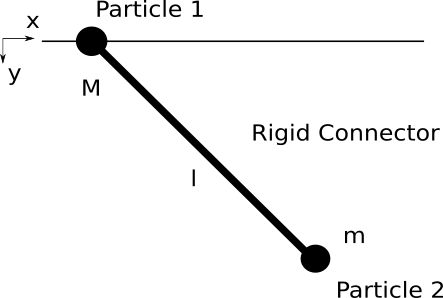
\includegraphics[width=0.5\linewidth]{PendulumDiagram.png}
			
	\section{The simplest case}
	We first consider the case where the support is moving with only constant velocity. This is already a case that is well studied as it just simplifies to a simple pendulum.
	
	The position vector of the pendulum bob can be written in terms of the generalized coordinate $\theta$ and the position vector of the support $ \vec{R} $.
	\[ \vec{r} = \vec{R} + l(sin(\theta) \hat{i} + cos(\theta) \hat{j} )\]
	
	Here, $ \vec{R} = Vt\hat{i} $
	Now,
	\[ \dot{\vec{r}}  = V\hat{i} + l\dot{\theta}( cos(\theta) \hat{i} - sin(\theta)\hat{j} )\]
	\[ \implies |\dot{\vec{r}}|^2 = V^2 + l^2\dot{\theta}^2 + 2Vlcos(\theta)\dot{\theta} \]	
	
	The Kinetic energy of the bob can be now written as 
	\[ T_2 = \frac{1}{2}m\dot{\vec{r}}^2 = \frac{m}{2}(V^2 + l^2\dot{\theta}^2 + 2Vlcos(\theta)\dot{\theta}) \]
	 The gravitational potential energy of the bob is
	\[ U_2 = -mglcos(\theta) \]
	 
	The kinetic energy of the support is,
	\[ T_1 = \frac{1}{2}MV^2 \]
	  
	The gravitational potential energy of the support is
	\[ U_1 = 0\]
	 
	The Lagrangian becomes,
	\[ L = T- U \]
	\[ \implies L  = \frac{m}{2}(V^2 + l^2\dot{\theta}^2 + 2Vlcos(\theta)\dot{\theta}) + mglcos(\theta) + \frac{1}{2}MV^2  \]
	
	\[ \therefore  L(\theta,\dot{\theta},t) = \frac{1}{2}m\dot{\vec{R}}^2 = \frac{m}{2}(V^2 + l^2\dot{\theta}^2 + 2Vlcos(\theta)\dot{\theta}) + mglcos(\theta) + \frac{1}{2}MV^2 \]
	
	Using Euler-Lagrange Equation,
	\[ \frac{d}{dt}\frac{\partial L}{\partial \dot{\theta}} = \frac{\partial L}{\partial \theta} \]
	\[ \implies \ddot{\theta} = -\frac{g}{l}\sin(\theta)  \]
	
	This is the same equation of motion as that of a simple pendulum with stationary support. This can be interpreted quite easily as the senario with constant motion of the support can be modelled as a simple pendulum on a moving vehicle. Since laws of Physics are same when moving under constant velocity we get the same equation of motion.
	
	Now, solving the equation,
	Let,
	\begin{equation}
		x_0 = \theta 	
	\end{equation}

	\begin{equation}\label{key}
		x_1 = \dot{\theta}
	\end{equation}

	$\therefore$ the equation of motion becomes,
	\[  \dot x_1 = -\frac{g}{l}sin(x_0) \]
	
	For small angles the above can be approximated using the sine approximation $ \sin \theta \approxeq \theta $
	\[ \therefore  \dot x_1 = -\frac{g}{l}x_0  \]
	The solution to this is Harmonic motion as expected.
	The Phase plots for various initial conditions are as shown.
	\begin{figure}[h!]
		\centering
		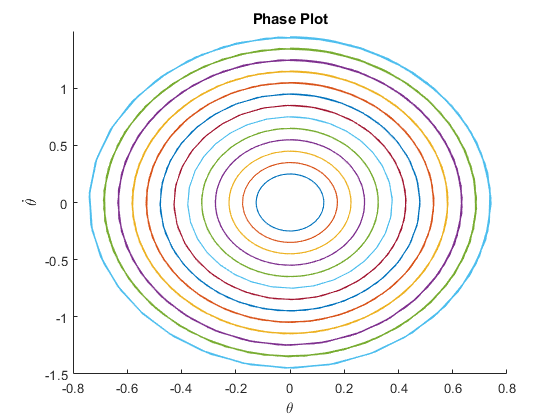
\includegraphics[width=0.5\linewidth]{Case1Plot1SmallAngles}
	\end{figure}

	
	When the approximation is not done, the numerical solution of the below equation gives the phase plot as:
	\[  \dot x_1 = -\frac{g}{l}sin(x_0) \]
	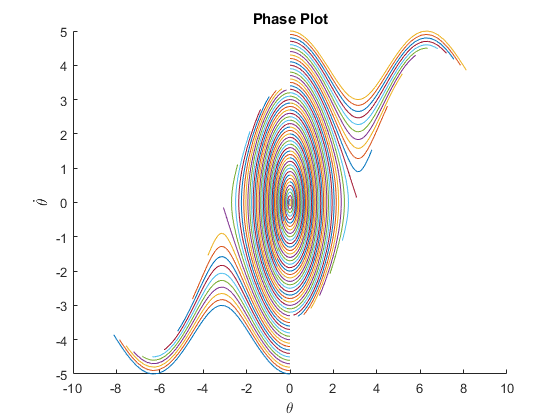
\includegraphics[width=0.5\linewidth]{Case1Plot2Directrix}



	\section{When the point of suspension is free}
	Let the suspension be given an initial velocity $ u $.
		
	The position vector of the pendulum bob can be written in terms of the generalized coordinate $\theta$ and the position vector of the support $ \vec{R} $ as earlier.
	\[ \vec{r} = \vec{R} + l(sin\theta \hat{i} + cos\theta \hat{j} )\]
	
	Here, $ \vec{R} $ does not have a simple equation like last time as the velocity of the support changes in accordance with the motion of the pendulum.
	\[ \vec{R} = x\hat{i} \]
	
	Now,
	\[ \dot{\vec{r}}  = \dot{x}\hat{i} + l\dot{\theta}( cos\theta \hat{i} - sin\theta\hat{j} ) \]
	\[ \implies |\dot{\vec{r}}|^2 = \dot{x}^2 + l^2 \dot{\theta}^2 + 2l\dot{x}\dot{\theta}\cos{\theta} \]	
	
	The Kinetic energy of the bob can be now written as 
	\[ T_2 = \frac{1}{2}m(\dot{x}^2 + l^2 \dot{\theta}^2 + 2l\dot{x}\dot{\theta}\cos{\theta}) \]
	
	The gravitational potential energy of the bob is
	\[ U_2 = -mglcos\theta \]
	
	The kinetic energy of the support is,
	\[ T_1 = \frac{1}{2}M\dot{x}^2 \]
	
	The gravitational potential energy of the support is
	\[ U_1 = 0\]
	
	The Lagrangian now becomes,
	\[ L = T -U \]
	\[ L =  \frac{1}{2}m(\dot{x}^2 + l^2 \dot{\theta}^2 + 2l\dot{x}\dot{\theta}\cos{\theta}) +  \frac{1}{2}M\dot{x}^2 + mglcos\theta  \]
	\[ \implies L(\theta,\dot{\theta},x,\dot{x},t) =  \frac{1}{2}m(\dot{x}^2 + l^2 \dot{\theta}^2 + 2l\dot{x}\dot{\theta}\cos{\theta}) +  \frac{1}{2}M\dot{x}^2 + mglcos\theta \]
	
	Now using Euler-Lagrange Equation.
	\begin{equation*}
		\frac{d}{dt}\frac{\partial L } {\partial \dot{\theta} } = \frac{\partial L}{\partial \theta} \tag{1}
	\end{equation*}
	\begin{equation*}
		\frac{d}{dt}\frac{\partial L } {\partial \dot{x} } = \frac{\partial L}{\partial x} \tag{2}
	\end{equation*}
	\begin{equation*}
		Equation 1 \implies ml^2\ddot{\theta} + ml\cos{\theta}\ddot{x}= -mgl\sin\theta	\tag{a}
	\end{equation*}
	\begin{equation*}
		Equation 2 \implies m\ddot{x} - ml\dot{\theta}^2\sin{\theta}+ ml\ddot{\theta} \cos\theta + M\ddot{x}	= 0 \tag{b}
	\end{equation*}
	The numerical solution for these two simultaneous equations have solutions of varied nature depending on the initial conditions.
	
	
	\subsection{Analytic Solution for Small Oscillations}
	For small oscillations where we approximate  follows,
	\[  \sin\theta \approxeq \theta\]
	\[  \cos\theta \approxeq 1 - \frac{\theta^2}{2}\]
	Substituting the above approximations into the Lagrangian obtained earlier and dropping the cubic and quadratic terms, we obtain,
	\[ L \approxeq \frac{1}{2}(M+m)\dot{x}^2 + ml\dot{x}\dot{\theta} + \frac{1}{2}ml^2\dot{\theta}^2 + mgl(1-\frac{\theta^2}{2}) \]
	 
	Now using Euler-Lagrange Equation.
	\begin{equation*}
	 	\frac{d}{dt}\frac{\partial L } {\partial \dot{\theta} } = \frac{\partial L}{\partial \theta} \tag{1}
	\end{equation*}
	\begin{equation*}
	 	\frac{d}{dt}\frac{\partial L } {\partial \dot{x} } = \frac{\partial L}{\partial x} \tag{2}
	\end{equation*}
	\begin{equation*}
	 	Equation 1 \implies ml\ddot{x}+ml^2\ddot{\theta}+mgl\theta=0	\tag{a}
	\end{equation*}
	\begin{equation*}
	 	Equation 2 \implies (M+m)\ddot{x}+ml\ddot{\theta}	= 0 \tag{b}
	\end{equation*}
 	Eliminating $ \ddot{x} $ from above equations,
 	\begin{equation*}
		ml^2\ddot{\theta}\biggr(1-\frac{m}{M+m}\biggr) + mgl\theta =0 	
    	\end{equation*}
 	The solution to this is that of a simple harmonic oscillator with frequency,
 	\[ \omega = \sqrt{\frac{g}{l}\biggr(\frac{m+M}{M}\biggr)} \]
 
 	We get the solution as,
 	\[ \theta(t) = A \cos(\omega t) + B \sin(\omega t) \]
 	\[ x(t) = Ct - \frac{ml}{m+M}(A \cos(\omega t) + B\sin(\omega t)) \]
 	\newpage
 
 	\section{Plots for Various Cases}
 	\centering
	Case 1:
	Same masses, no initial velocity to support and small initial angular velocity.
	\newline
	
	\begin{figure}[h!]
		\graphicspath{{./SmallOscillations/S1} }
		\centering
		\begin{subfigure}[b]{0.48\linewidth}
			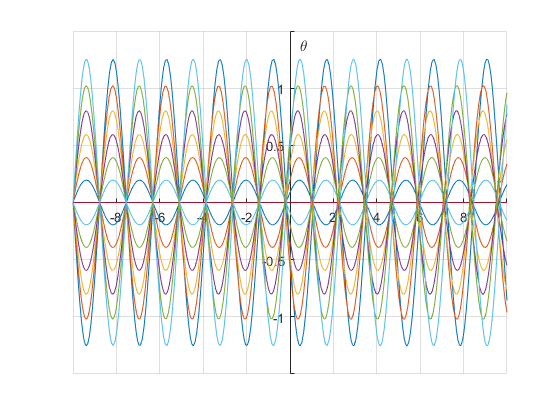
\includegraphics[width=\linewidth]{./F1.png}
		\end{subfigure}
		\begin{subfigure}[b]{0.48\linewidth}
			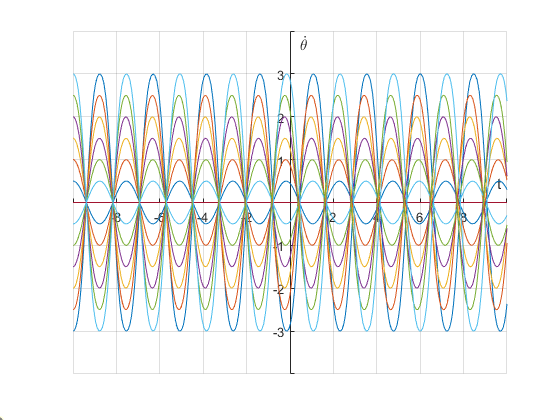
\includegraphics[width=\linewidth]{./F2.png}
		\end{subfigure}
	\end{figure}
	
	
	\begin{figure}[h!]
		\graphicspath{{./SmallOscillations/S1} }
		\centering
		\begin{subfigure}[b]{0.48\linewidth}
			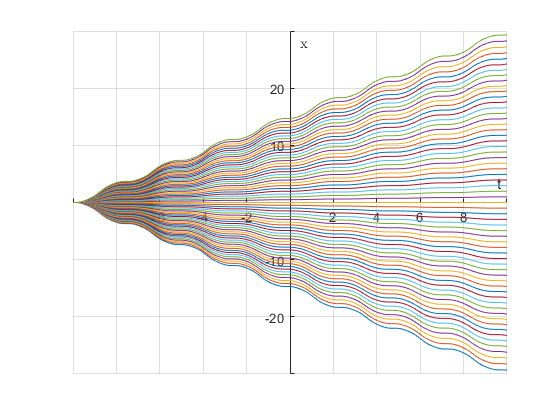
\includegraphics[width=\linewidth]{./F3.png}
		\end{subfigure}	
		\begin{subfigure}[b]{0.48\linewidth}
			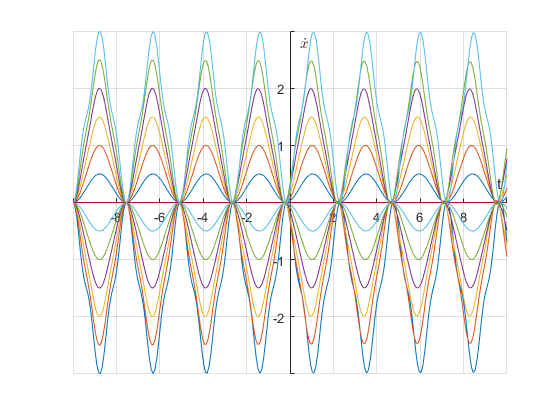
\includegraphics[width=\linewidth]{./F4.png}
		\end{subfigure}
    	\end{figure}
	
	
	\begin{figure}[h!]
	\graphicspath{{./SmallOscillations/S1} }
	\centering
		\begin{subfigure}[b]{0.48\linewidth}
			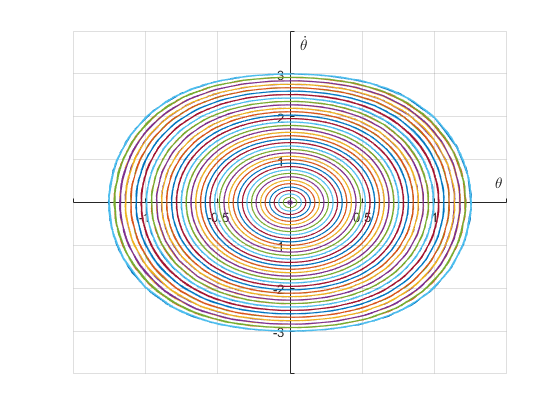
\includegraphics[width=\linewidth]{./F5.png}
		\end{subfigure}		
		\begin{subfigure}[b]{0.48\linewidth}
			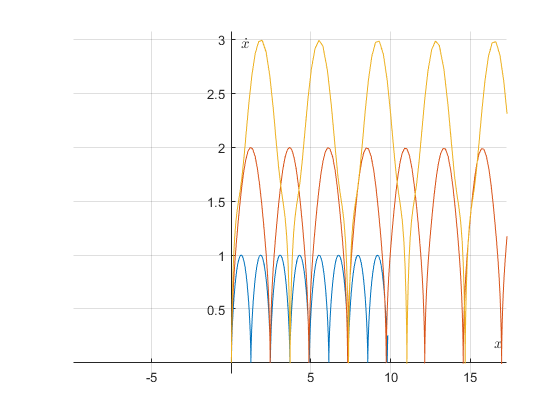
\includegraphics[width=\linewidth]{./F6.png}
		\end{subfigure}
	\end{figure}
	\newpage
	
	Case 2:
	Same masses, no initial velocity to support and small angular displacement.	
	\graphicspath{{./SmallOscillations/S2} }
	\begin{figure}[h!]
		\centering
		\begin{subfigure}[b]{0.48\linewidth}
			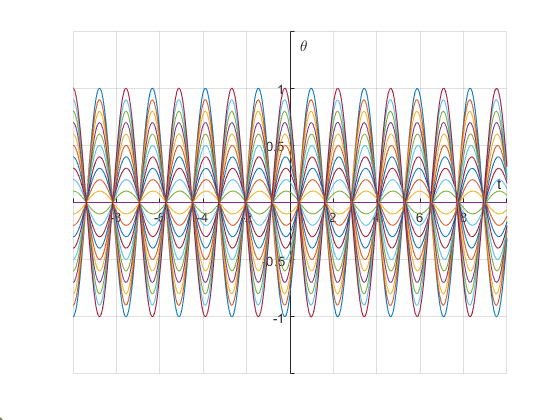
\includegraphics[width=\linewidth]{./SmallOscillations/S2/F1.png}
		\end{subfigure}
		\begin{subfigure}[b]{0.48\linewidth}
			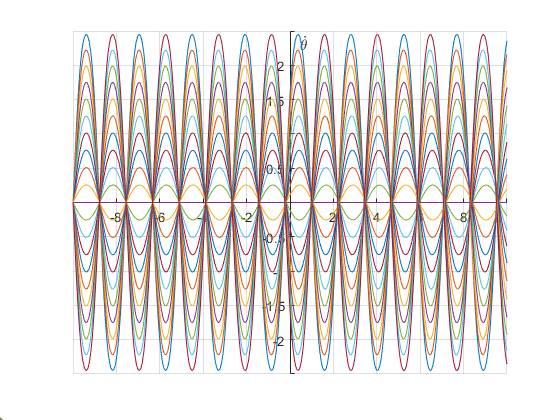
\includegraphics[width=\linewidth]{./SmallOscillations/S2/F2.png}
		\end{subfigure}
	\end{figure}
	
	\begin{figure}[h!]
		\graphicspath{{./SmallOscillations/S1} }
		\centering
		\begin{subfigure}[b]{0.48\linewidth}
			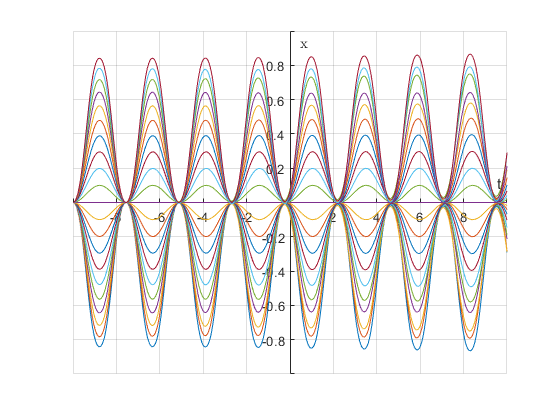
\includegraphics[width=\linewidth]{./SmallOscillations/S2/F3.png}
		\end{subfigure}
		\begin{subfigure}[b]{0.48\linewidth}
			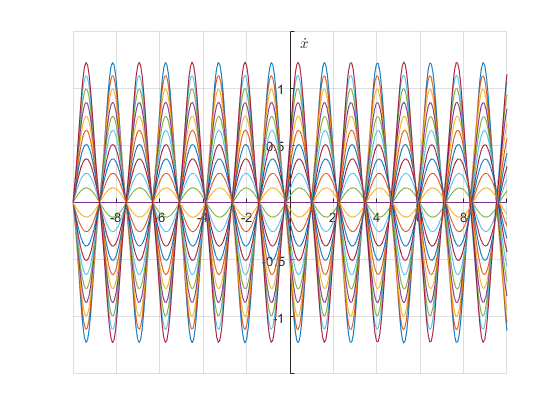
\includegraphics[width=\linewidth]{./SmallOscillations/S2/F4.png}
		\end{subfigure}
	\end{figure}
	
	\begin{figure}[h!]
		\graphicspath{{./SmallOscillations/S1} }
		\centering
		\begin{subfigure}[b]{0.48\linewidth}
			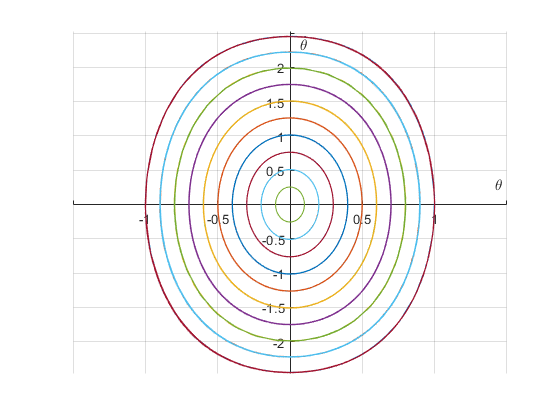
\includegraphics[width=\linewidth]{./SmallOscillations/S2/F5.png}
		\end{subfigure}
		\begin{subfigure}[b]{0.48\linewidth}
			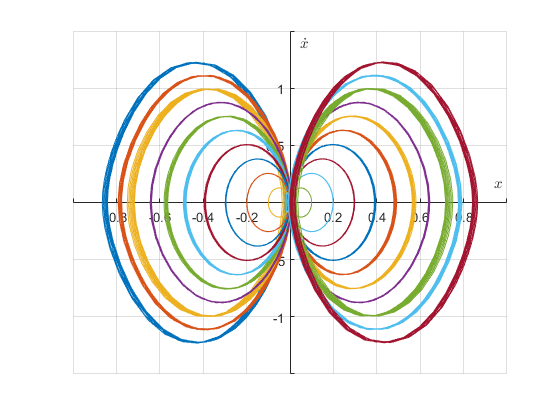
\includegraphics[width=\linewidth]{./SmallOscillations/S2/F6.png}
		\end{subfigure}
	\end{figure}
	\newpage

	
	Case 3:
	Same masses, initial velocity to support and small initial angular velocity.
	\graphicspath{{./SmallOscillations/S3} }
	\begin{figure}[h!]
		\centering
		\begin{subfigure}[b]{0.48\linewidth}
			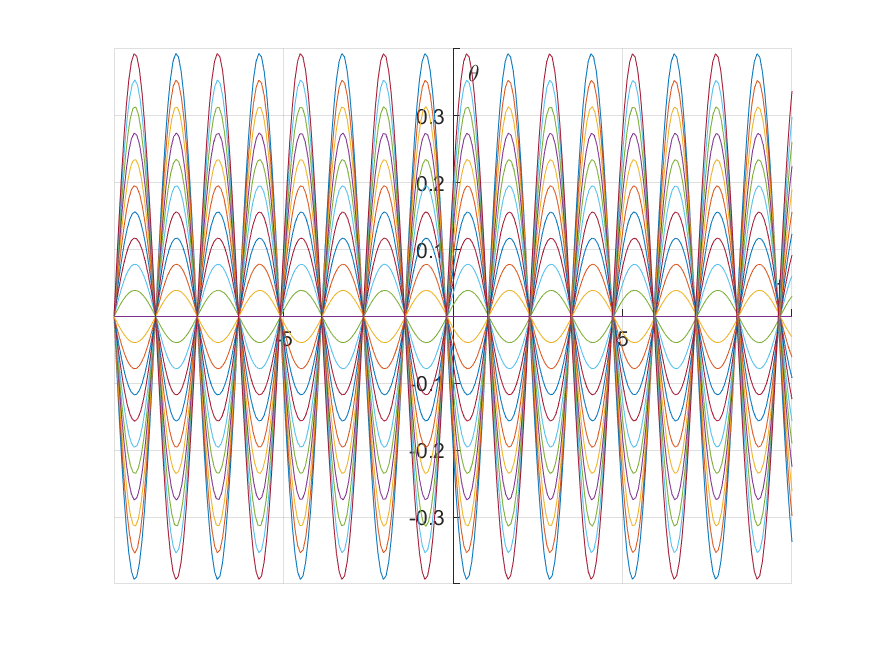
\includegraphics[width=\linewidth]{./SmallOscillations/S3/F1.png}
		\end{subfigure}
		\begin{subfigure}[b]{0.48\linewidth}
			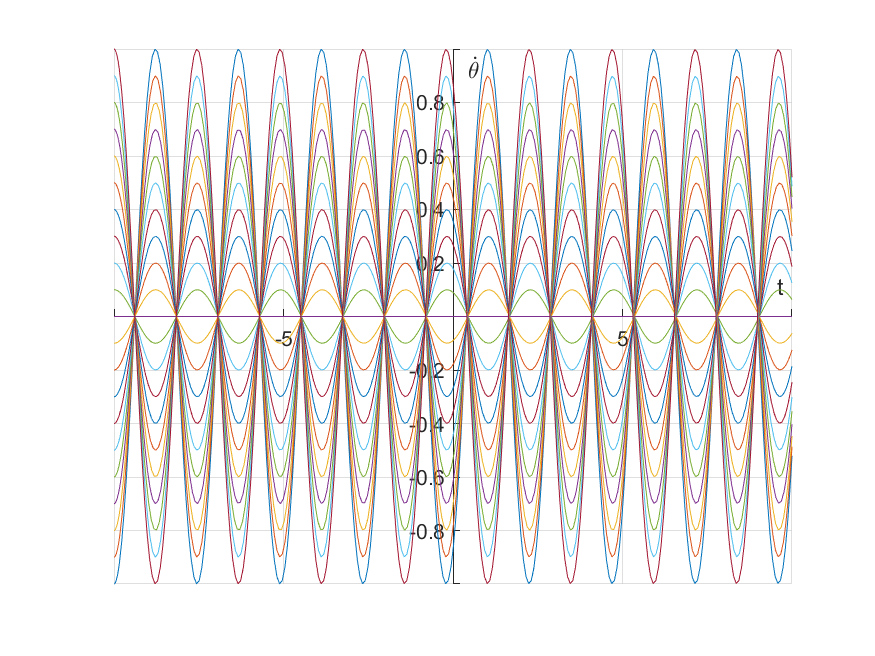
\includegraphics[width=\linewidth]{./SmallOscillations/S3/F2.png}
		\end{subfigure}
	\end{figure}

	\begin{figure}[h!]
		\centering
		\begin{subfigure}[b]{0.48\linewidth}
			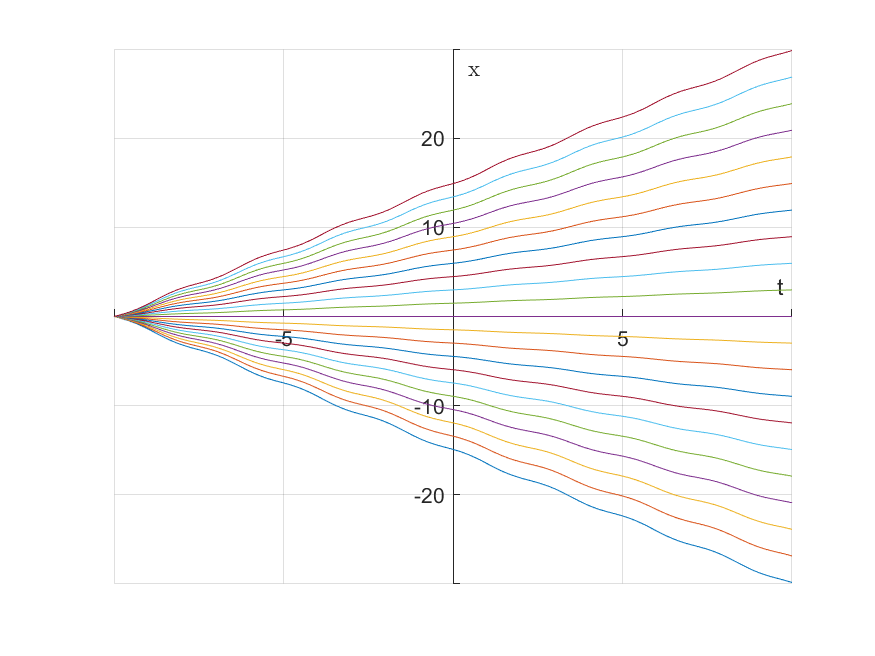
\includegraphics[width=\linewidth]{./SmallOscillations/S3/F3.png}
		\end{subfigure}
		\begin{subfigure}[b]{0.48\linewidth}
			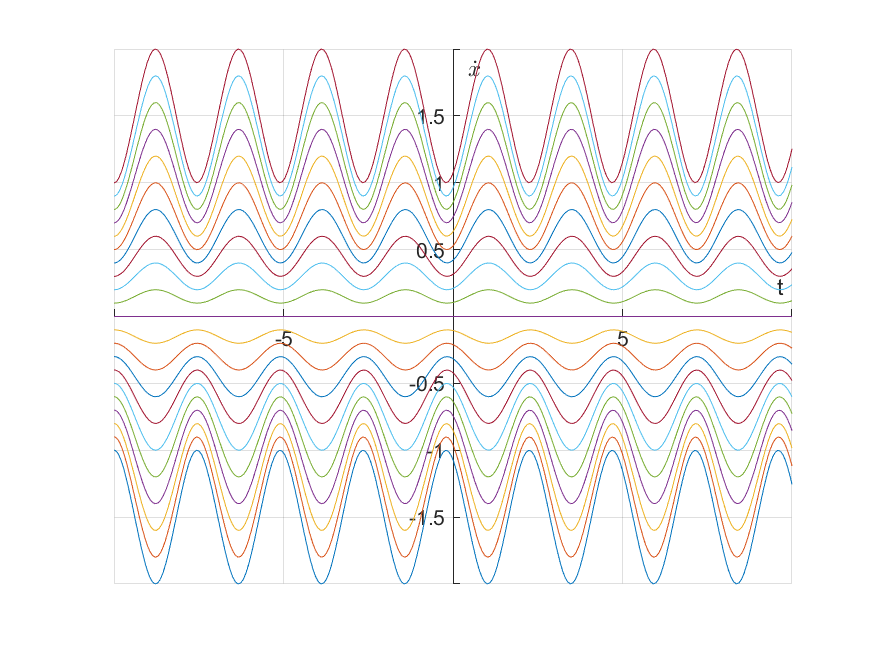
\includegraphics[width=\linewidth]{./SmallOscillations/S3/F4.png}
		\end{subfigure}
	\end{figure}

	\begin{figure}[h!]
		\centering
		\begin{subfigure}[b]{0.48\linewidth}
			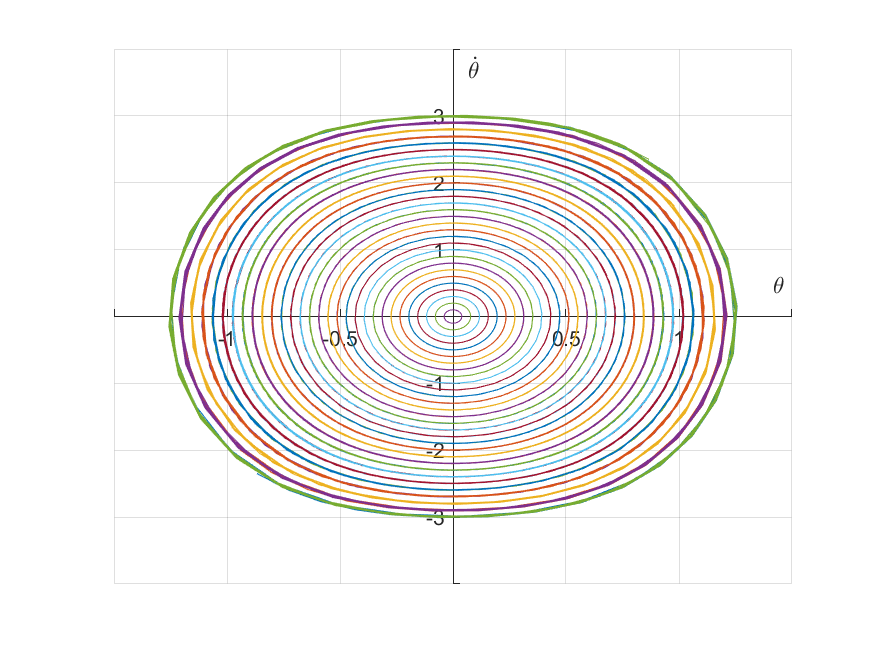
\includegraphics[width=\linewidth]{./SmallOscillations/S3/F5.png}
		\end{subfigure}
		\begin{subfigure}[b]{0.48\linewidth}
			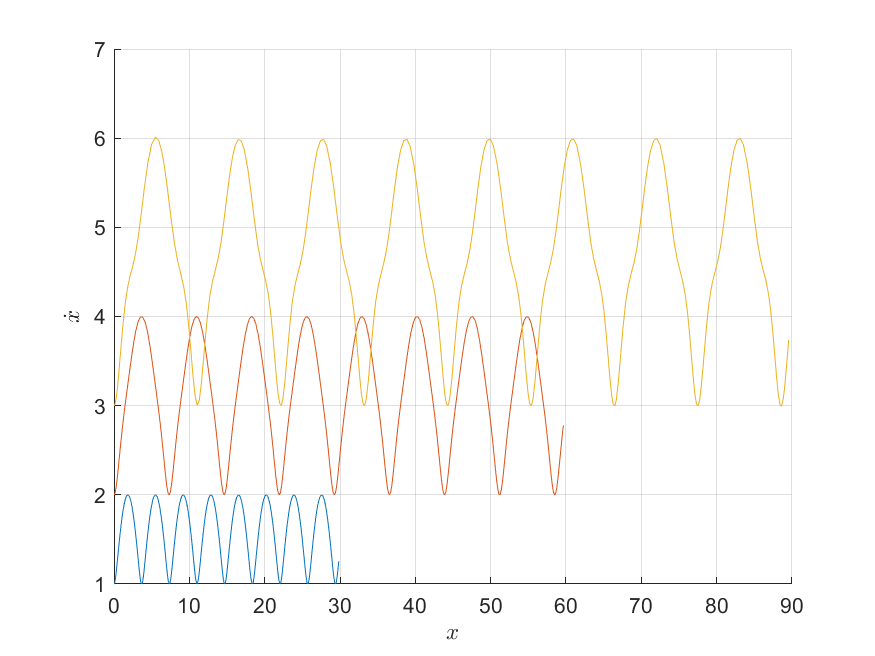
\includegraphics[width=\linewidth]{./SmallOscillations/S3/F6.png}
		\end{subfigure}
	\end{figure}
	\newpage
	
	
	Case 4:
	Same masses, initial velocity to support and small angular displacement.
	\begin{figure}[h!]
		\centering
		\begin{subfigure}[b]{0.48\linewidth}
			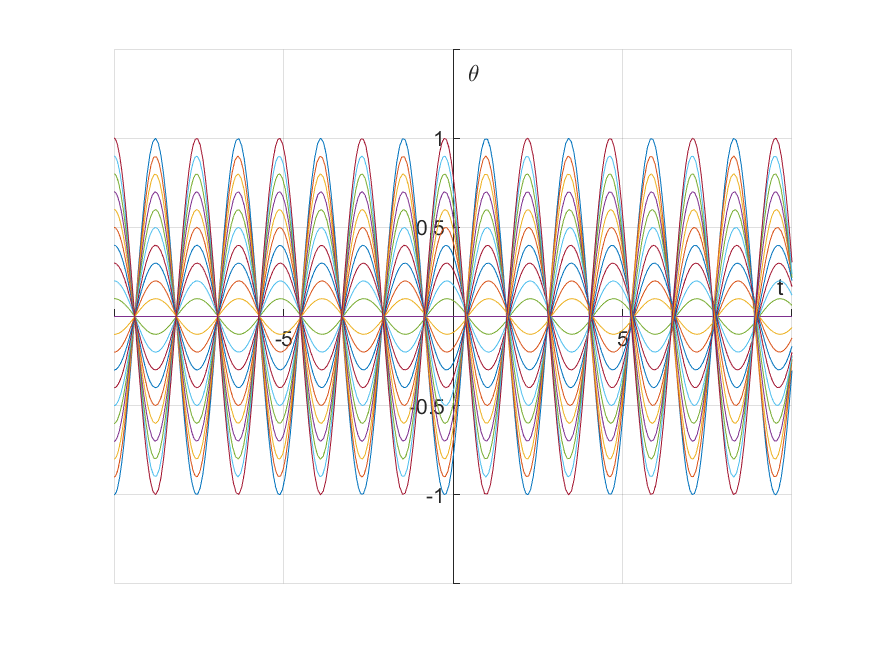
\includegraphics[width=\linewidth]{./SmallOscillations/S4/F1.png}
		\end{subfigure}
		\begin{subfigure}[b]{0.48\linewidth}
			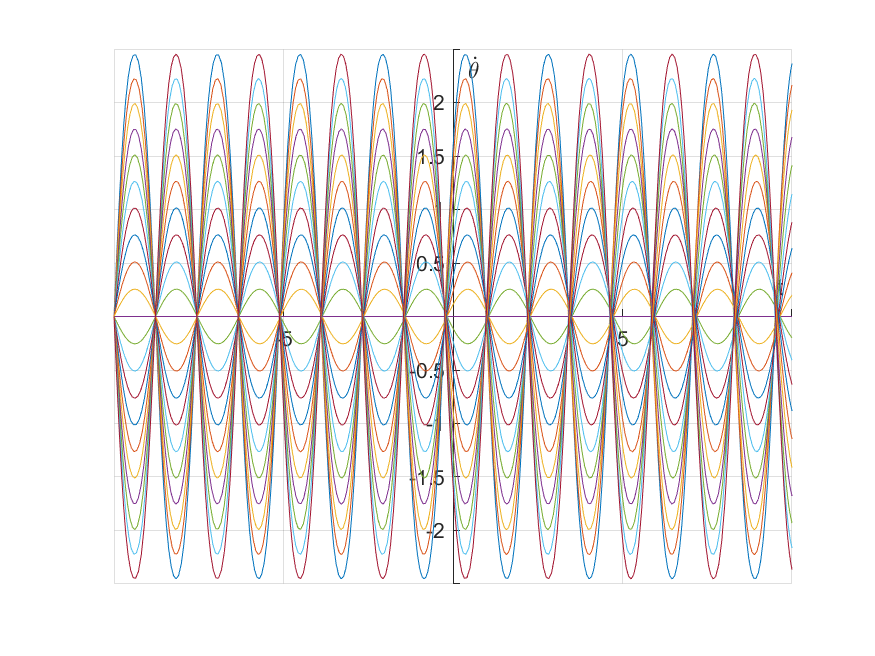
\includegraphics[width=\linewidth]{./SmallOscillations/S4/F2.png}
		\end{subfigure}
	\end{figure}
	
	\begin{figure}[h!]
		\centering
		\begin{subfigure}[b]{0.48\linewidth}
			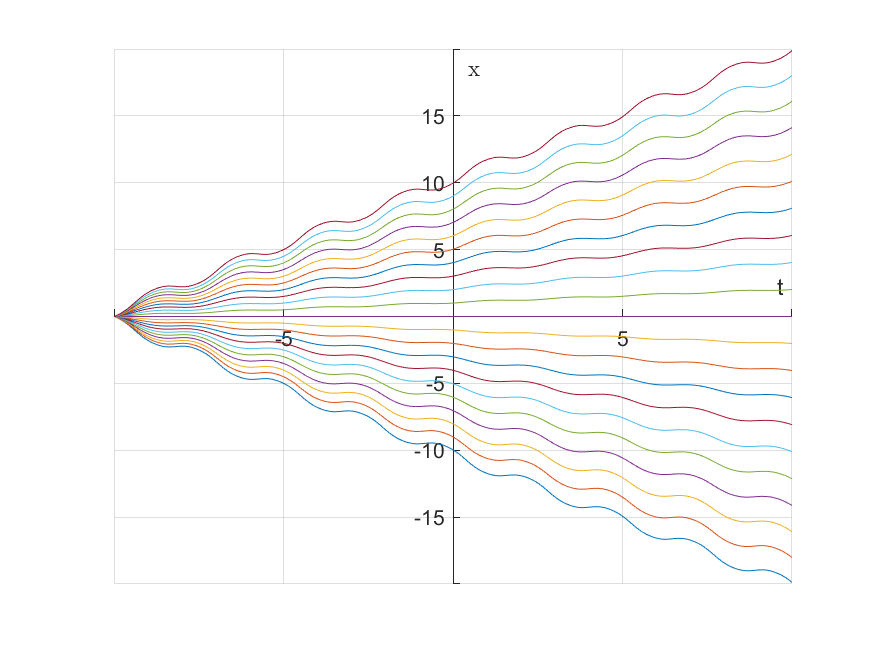
\includegraphics[width=\linewidth]{./SmallOscillations/S4/F3.png}
		\end{subfigure}
		\begin{subfigure}[b]{0.48\linewidth}
			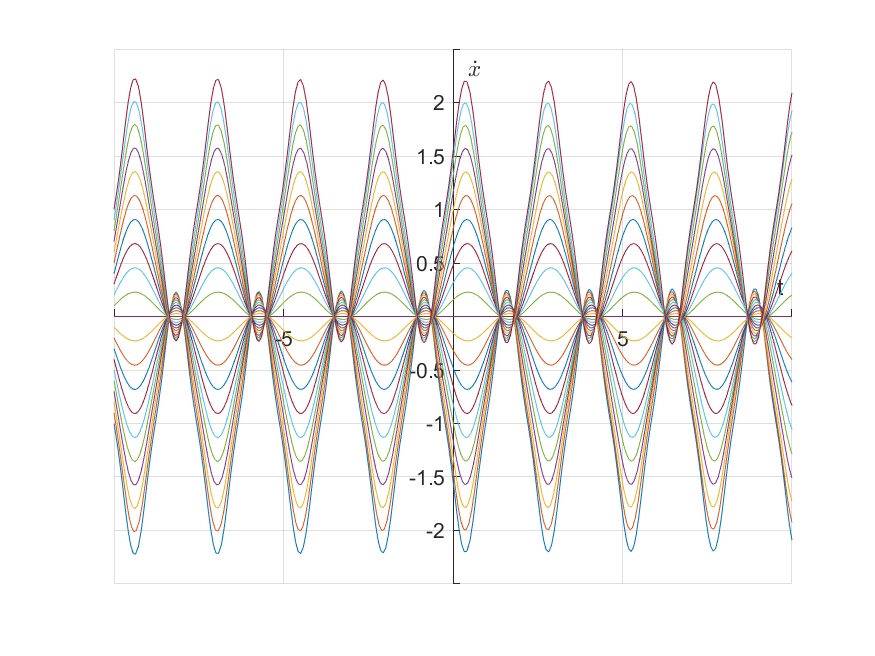
\includegraphics[width=\linewidth]{./SmallOscillations/S4/F4.png}
		\end{subfigure}
	\end{figure}
	
	\begin{figure}[h!]
		\centering
		\begin{subfigure}[b]{0.48\linewidth}
			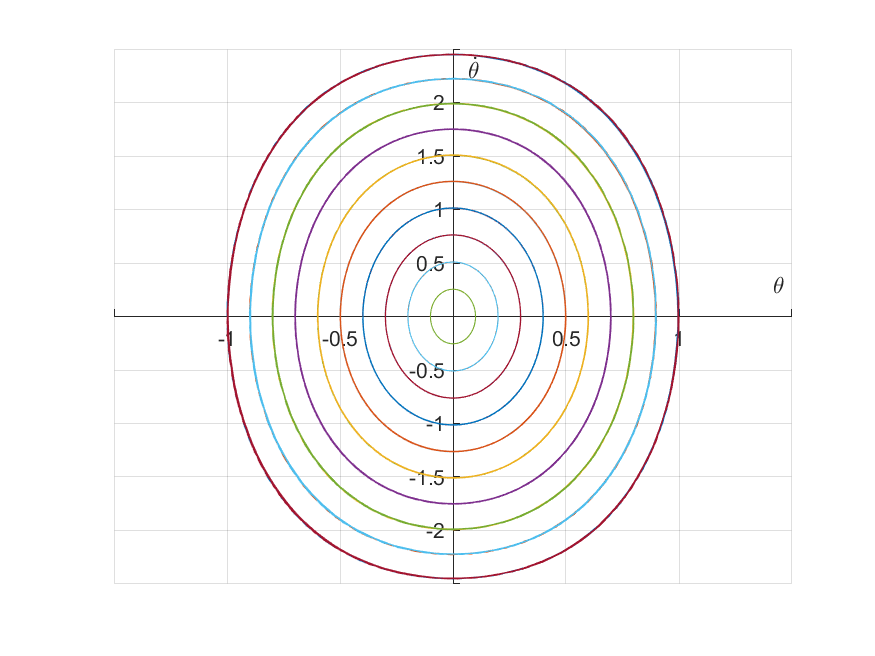
\includegraphics[width=\linewidth]{./SmallOscillations/S4/F5.png}
		\end{subfigure}
		\begin{subfigure}[b]{0.48\linewidth}
			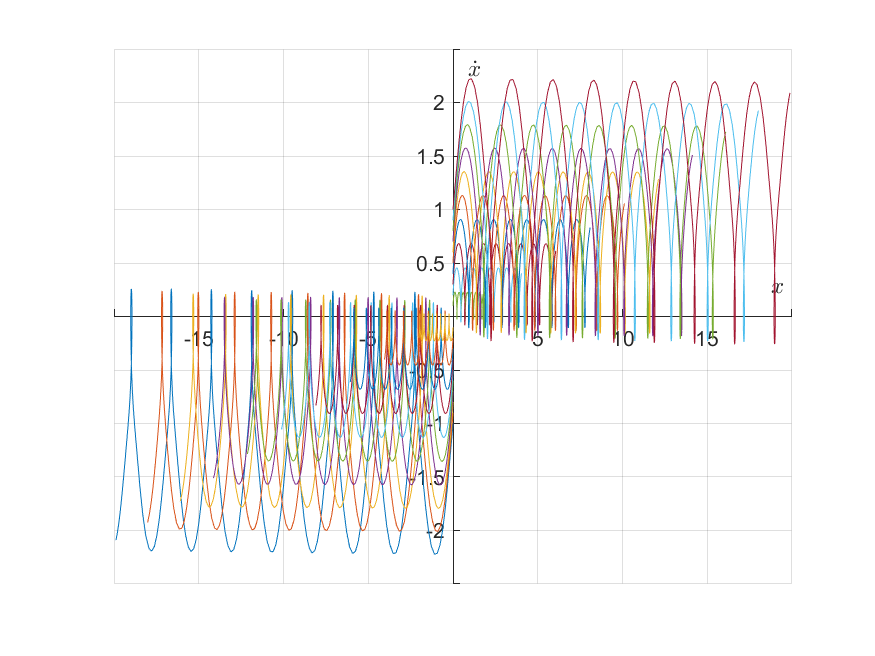
\includegraphics[width=\linewidth]{./SmallOscillations/S4/F6.png}
		\end{subfigure}
	\end{figure}
	\newpage
	
	Case 5:
	Large support mass, no initial velocity to support and small initial angular velocity.
	\begin{figure}[h!]
		\centering
		\begin{subfigure}[b]{0.48\linewidth}
			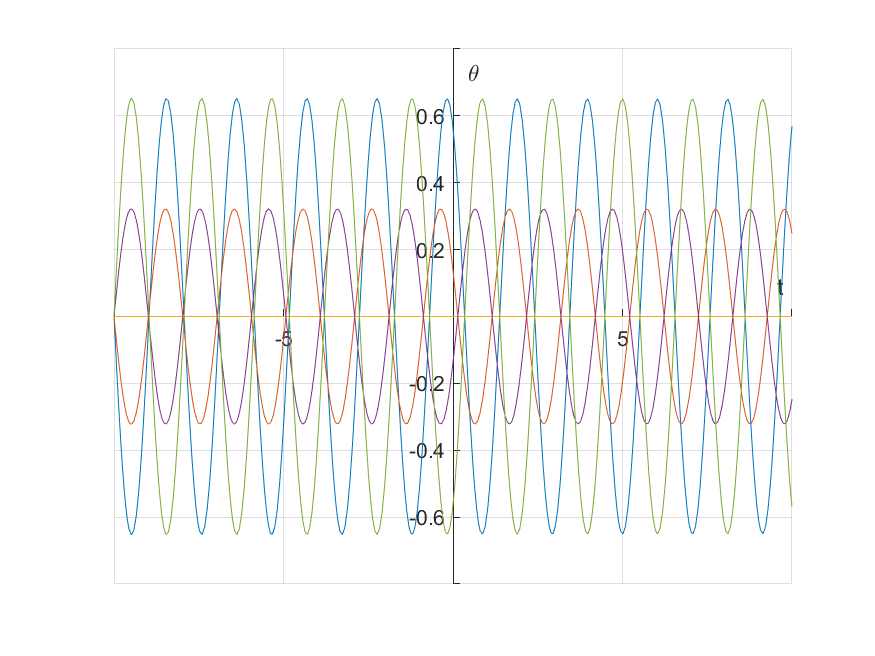
\includegraphics[width=\linewidth]{./SmallOscillations/S5/F1.png}
		\end{subfigure}
		\begin{subfigure}[b]{0.48\linewidth}
			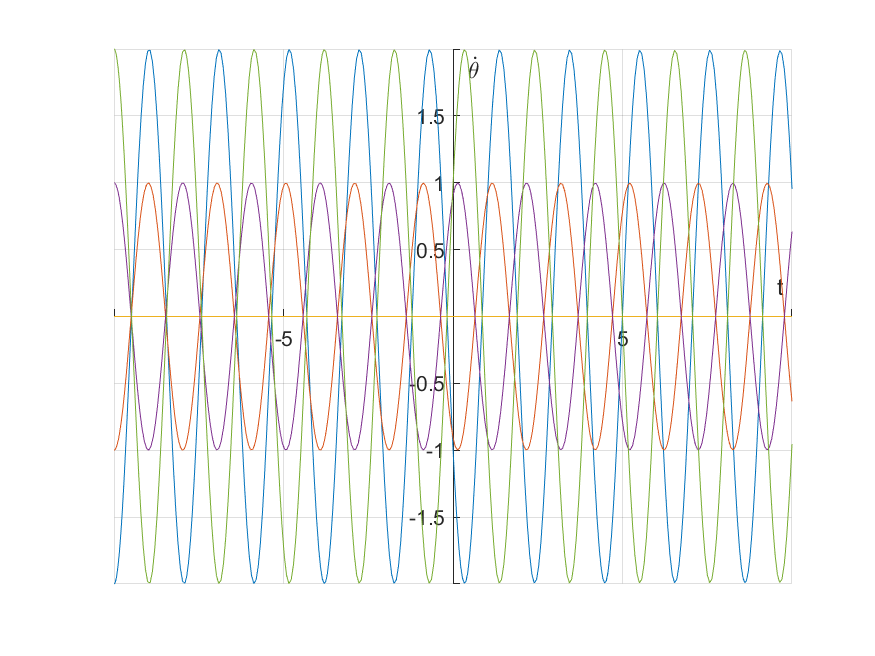
\includegraphics[width=\linewidth]{./SmallOscillations/S5/F2.png}
		\end{subfigure}
	\end{figure}
	
	\begin{figure}[h!]
		\centering
		\begin{subfigure}[b]{0.48\linewidth}
			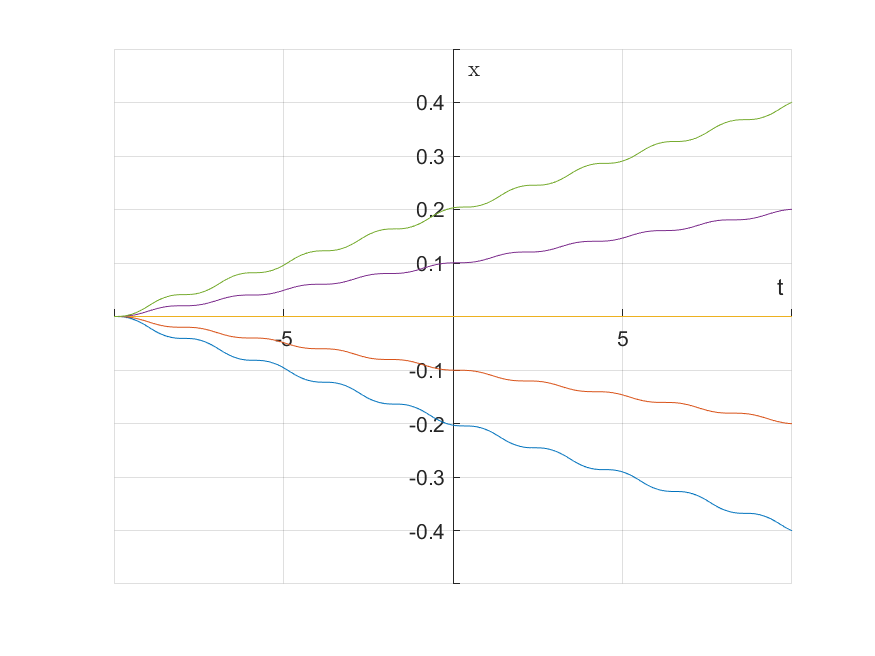
\includegraphics[width=\linewidth]{./SmallOscillations/S5/F3.png}
		\end{subfigure}
		\begin{subfigure}[b]{0.48\linewidth}
			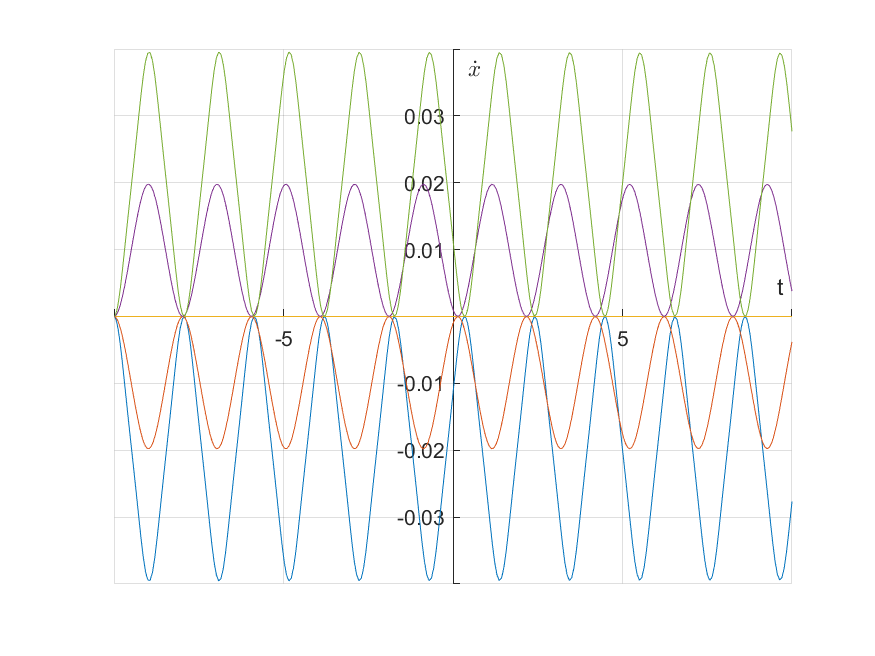
\includegraphics[width=\linewidth]{./SmallOscillations/S5/F4.png}
		\end{subfigure}
	\end{figure}
	
	\begin{figure}[h!]
		\centering
		\begin{subfigure}[b]{0.48\linewidth}
			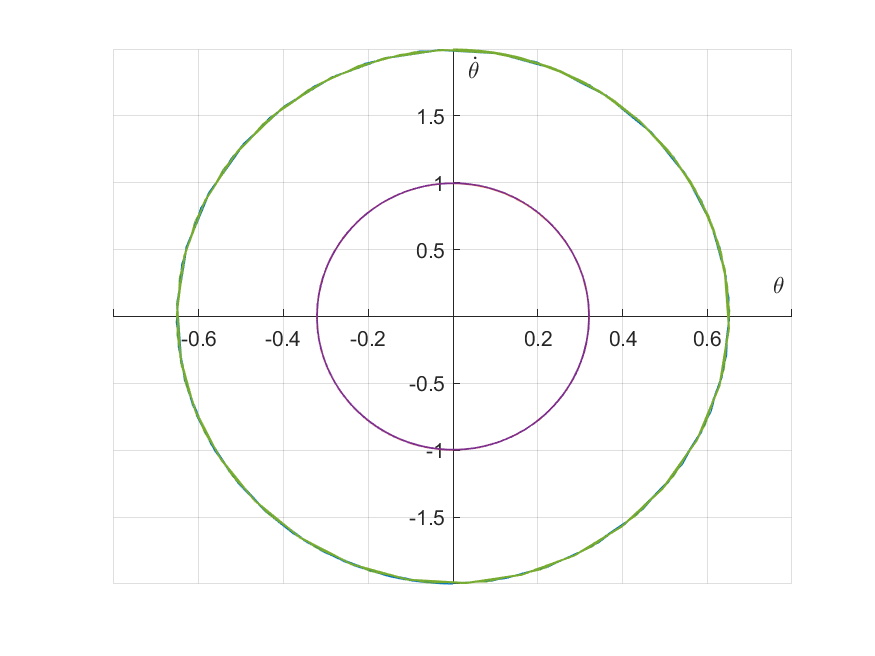
\includegraphics[width=\linewidth]{./SmallOscillations/S5/F5.png}
		\end{subfigure}
		\begin{subfigure}[b]{0.48\linewidth}
			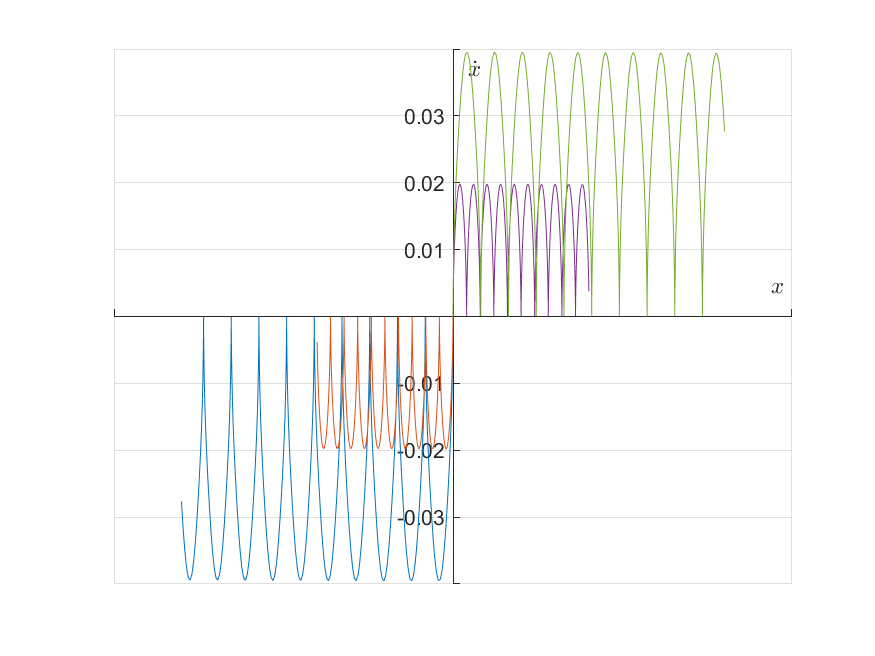
\includegraphics[width=\linewidth]{./SmallOscillations/S5/F6.png}
		\end{subfigure}
	\end{figure}
	\newpage
	
	Case 6:
	Large support mass, no initial velocity to support and small angular displacement.
	\begin{figure}[h!]
		\centering
		\begin{subfigure}[b]{0.48\linewidth}
			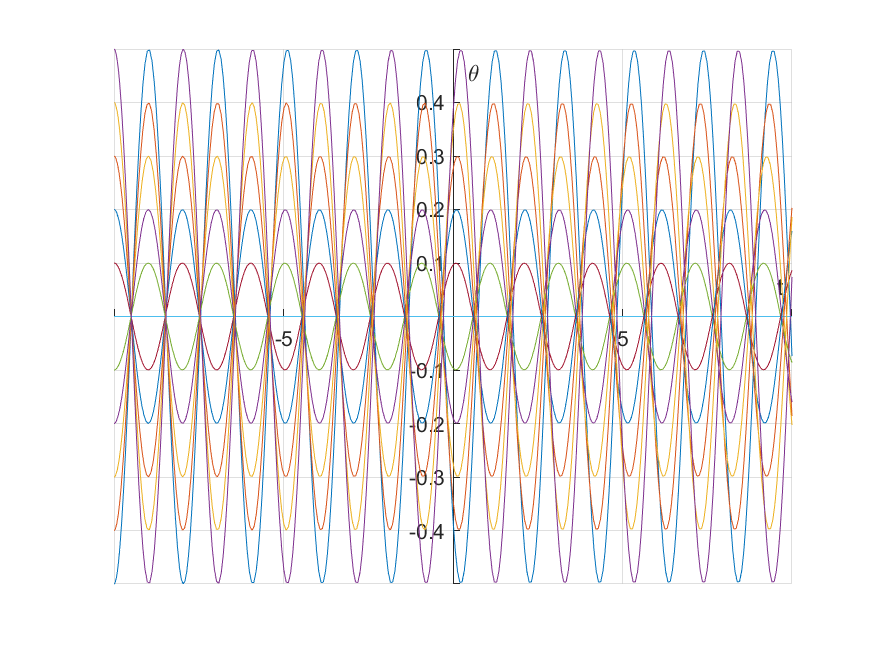
\includegraphics[width=\linewidth]{./SmallOscillations/S6/F1.png}
		\end{subfigure}
		\begin{subfigure}[b]{0.48\linewidth}
			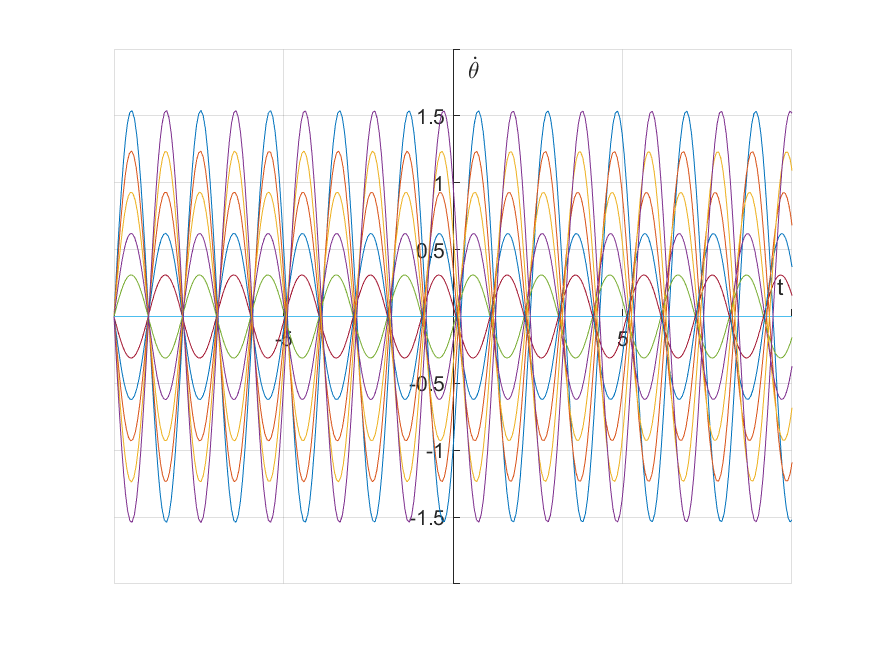
\includegraphics[width=\linewidth]{./SmallOscillations/S6/F2.png}
		\end{subfigure}
	\end{figure}
	
	\begin{figure}[h!]
		\centering
		\begin{subfigure}[b]{0.48\linewidth}
			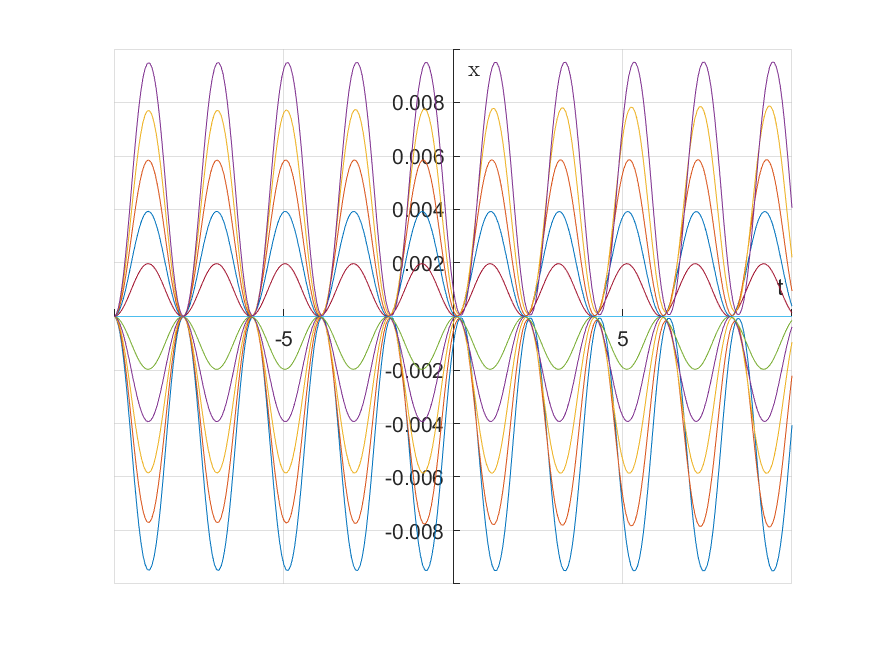
\includegraphics[width=\linewidth]{./SmallOscillations/S6/F3.png}
		\end{subfigure}
		\begin{subfigure}[b]{0.48\linewidth}
			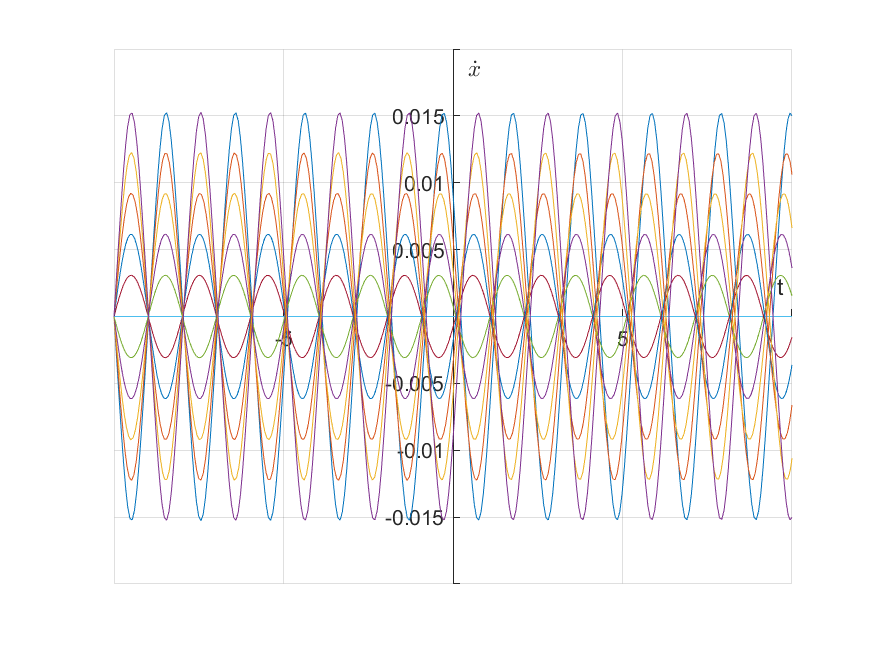
\includegraphics[width=\linewidth]{./SmallOscillations/S6/F4.png}
		\end{subfigure}
	\end{figure}
	
	\begin{figure}[h!]
		\centering
		\begin{subfigure}[b]{0.48\linewidth}
			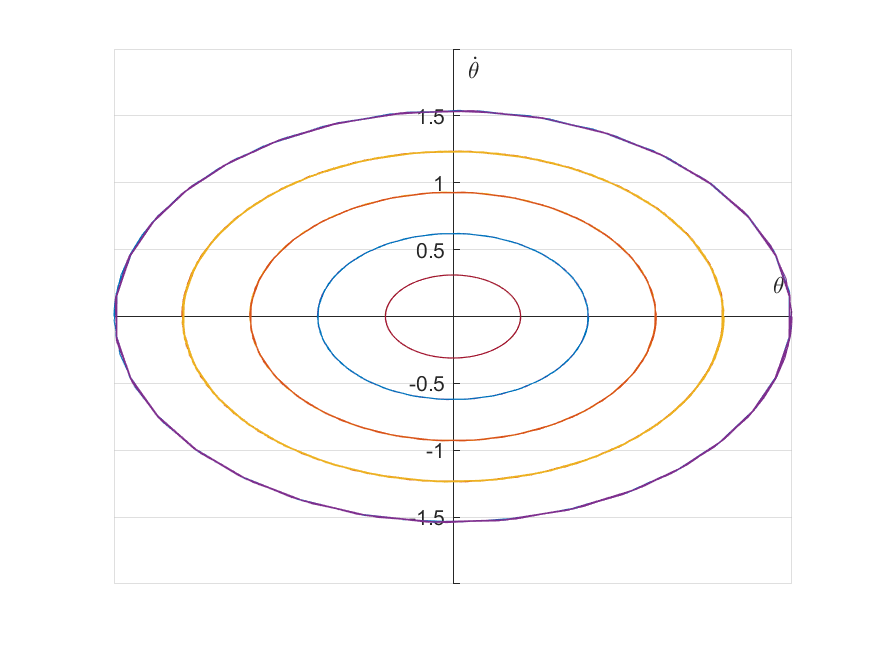
\includegraphics[width=\linewidth]{./SmallOscillations/S6/F5.png}
		\end{subfigure}
		\begin{subfigure}[b]{0.48\linewidth}
			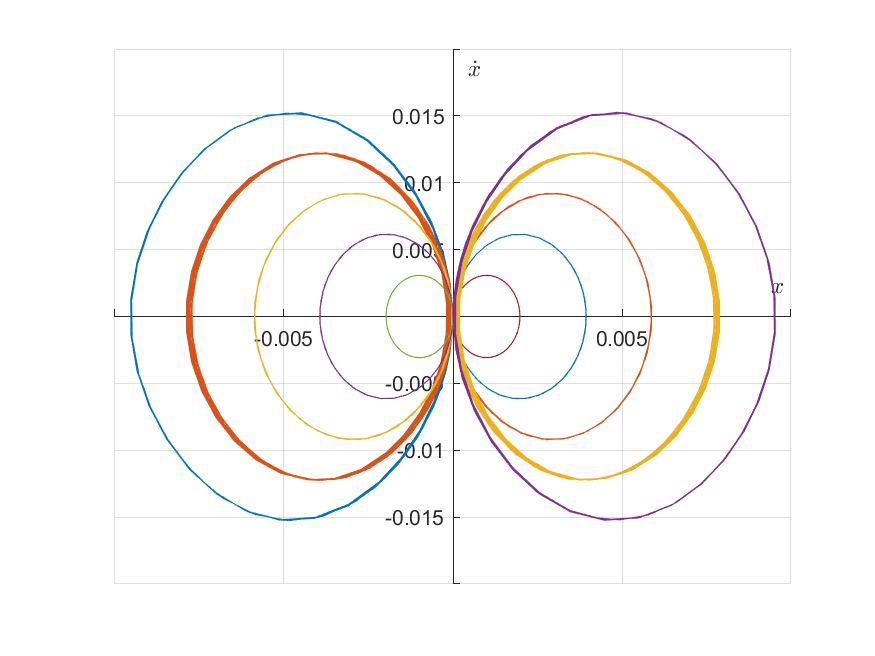
\includegraphics[width=\linewidth]{./SmallOscillations/S6/F6.png}
		\end{subfigure}
	\end{figure}
	\newpage	
	
	Case 7:
	Large support mass, initial velocity to support and small initial angular velocity.
	\begin{figure}[h!]
		\centering
		\begin{subfigure}[b]{0.48\linewidth}
			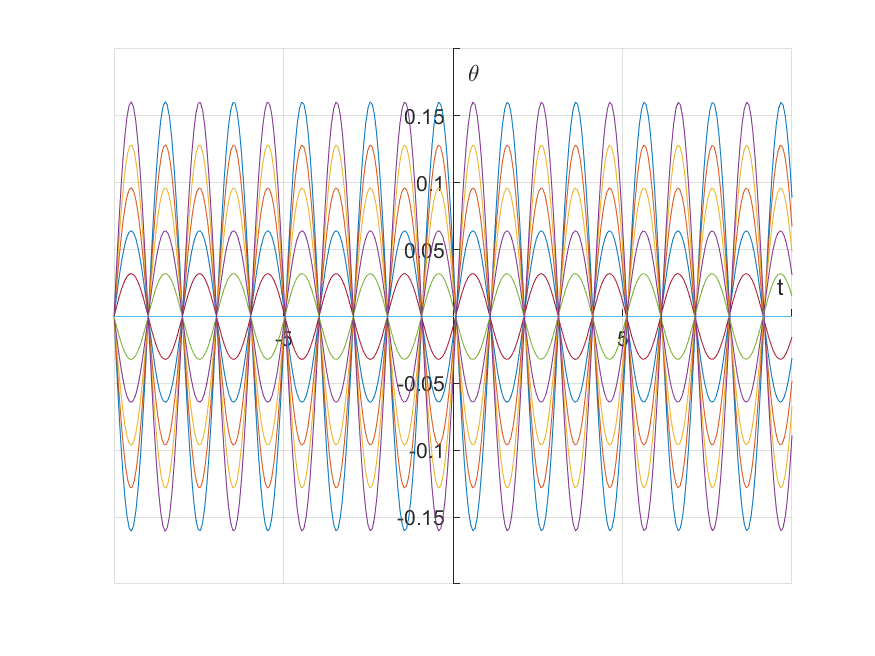
\includegraphics[width=\linewidth]{./SmallOscillations/S7/F1.png}
		\end{subfigure}
		\begin{subfigure}[b]{0.48\linewidth}
			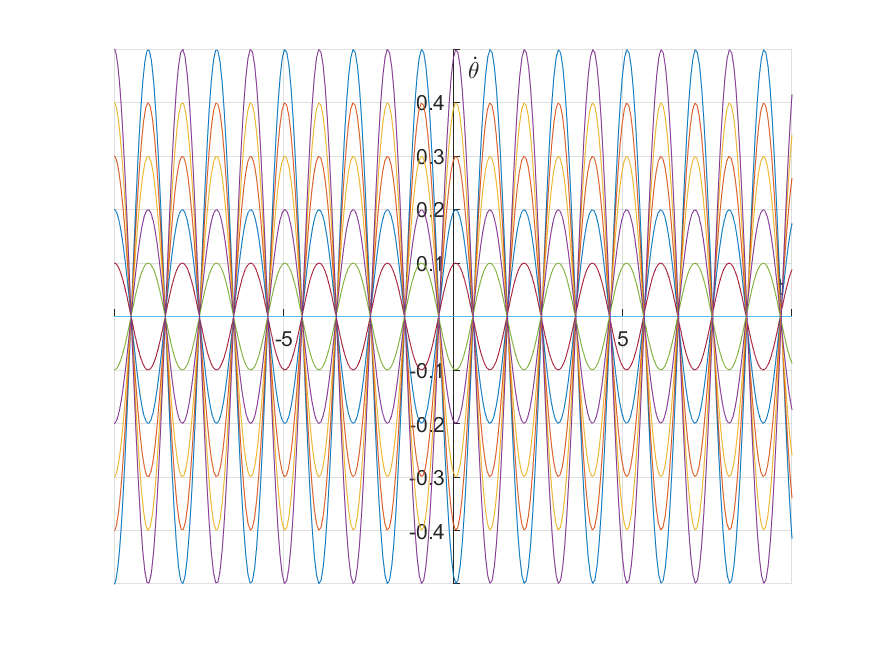
\includegraphics[width=\linewidth]{./SmallOscillations/S7/F2.png}
		\end{subfigure}
	\end{figure}
	
	\begin{figure}[h!]
		\centering
		\begin{subfigure}[b]{0.48\linewidth}
			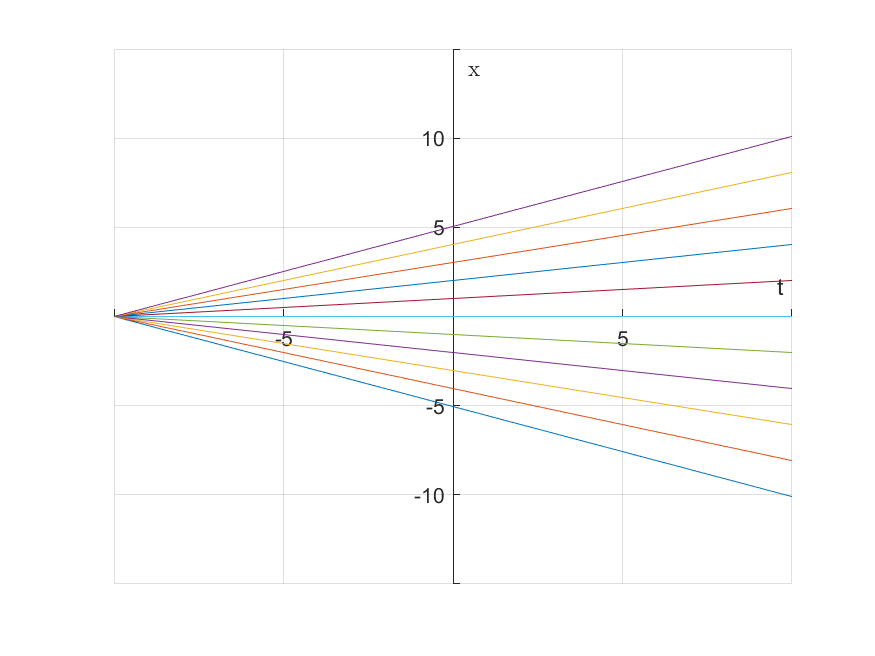
\includegraphics[width=\linewidth]{./SmallOscillations/S7/F3.png}
		\end{subfigure}
		\begin{subfigure}[b]{0.48\linewidth}
			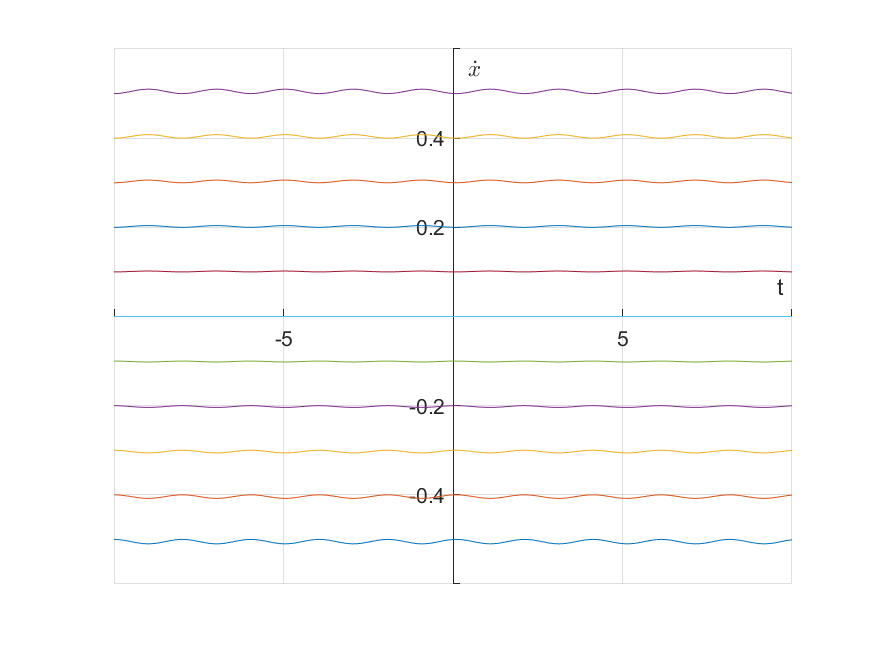
\includegraphics[width=\linewidth]{./SmallOscillations/S7/F4.png}
		\end{subfigure}
	\end{figure}
	
	\begin{figure}[h!]
		\centering
		\begin{subfigure}[b]{0.48\linewidth}
			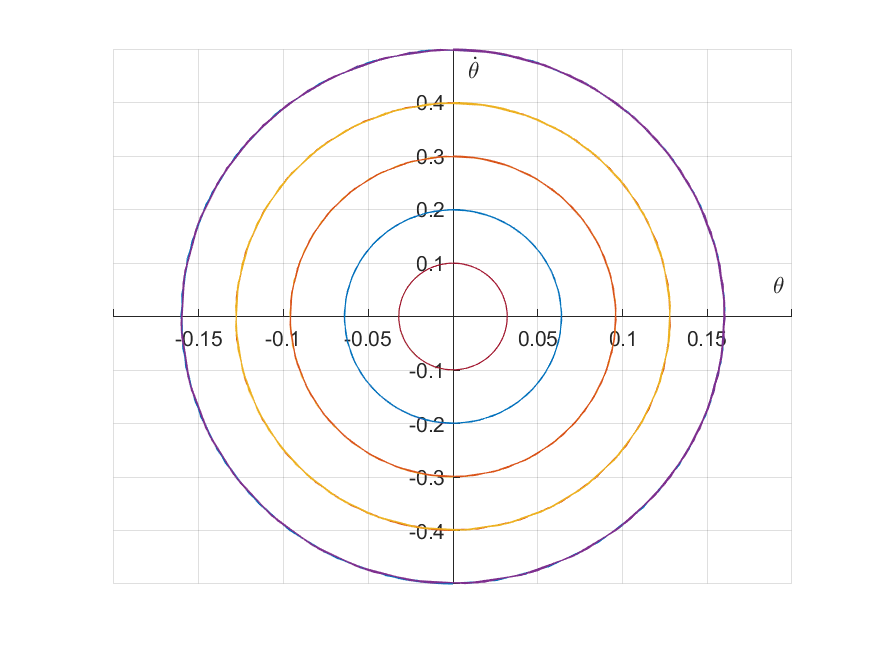
\includegraphics[width=\linewidth]{./SmallOscillations/S7/F5.png}
		\end{subfigure}
		\begin{subfigure}[b]{0.48\linewidth}
			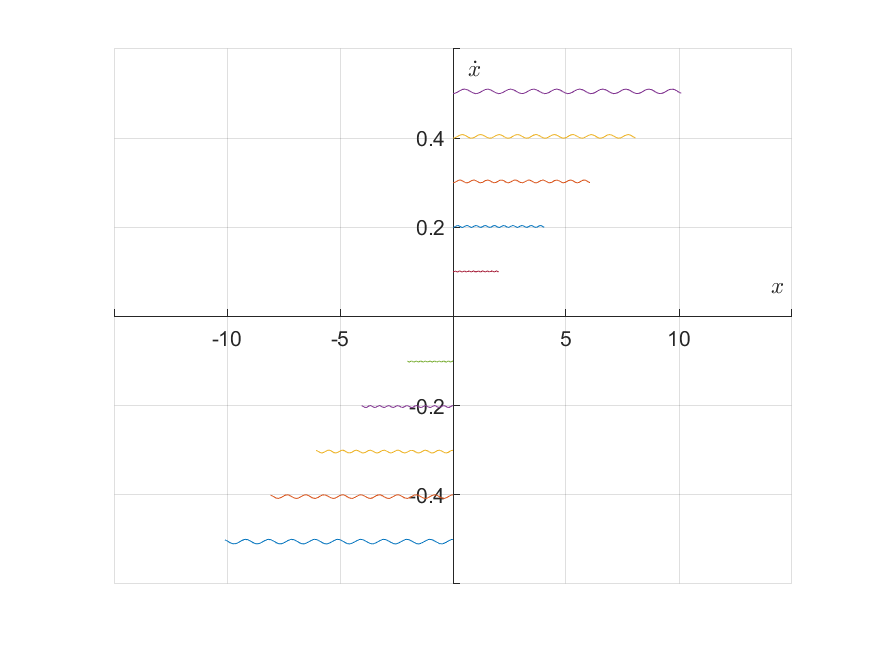
\includegraphics[width=\linewidth]{./SmallOscillations/S7/F6.png}
		\end{subfigure}
	\end{figure}
	\newpage
	
	Case 8:
	Large support mass, initial velocity to support and small angular displacement.
	\begin{figure}[h!]
		\centering
		\begin{subfigure}[b]{0.48\linewidth}
			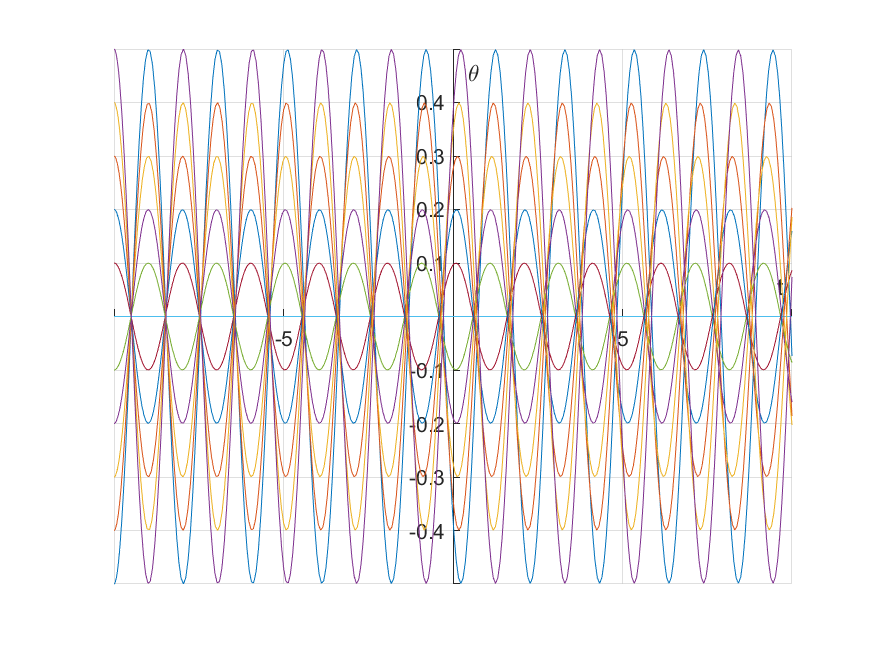
\includegraphics[width=\linewidth]{./SmallOscillations/S8/F1.png}
		\end{subfigure}
		\begin{subfigure}[b]{0.48\linewidth}
			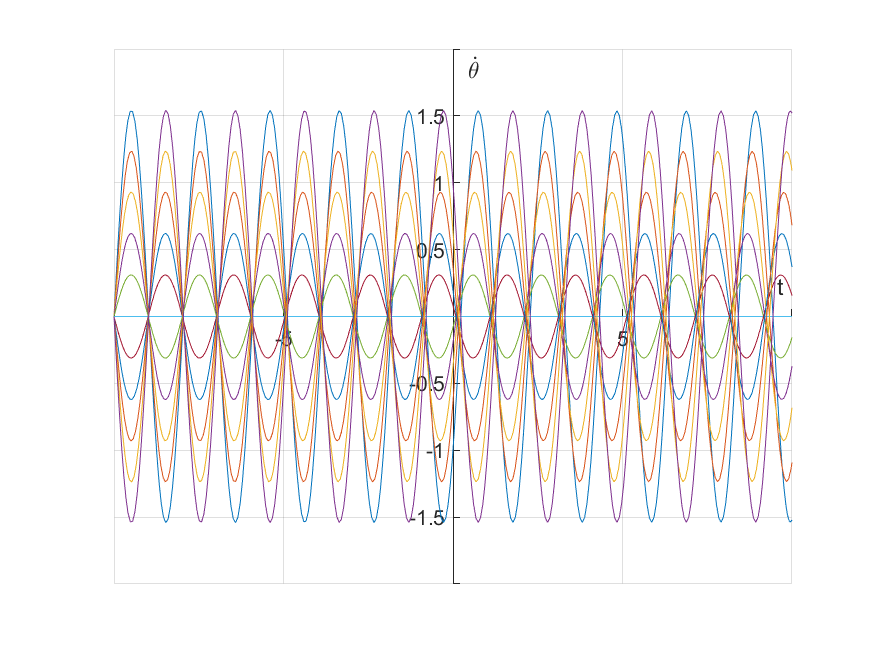
\includegraphics[width=\linewidth]{./SmallOscillations/S8/F2.png}
		\end{subfigure}
	\end{figure}
	
	\begin{figure}[h!]
		\centering
		\begin{subfigure}[b]{0.48\linewidth}
			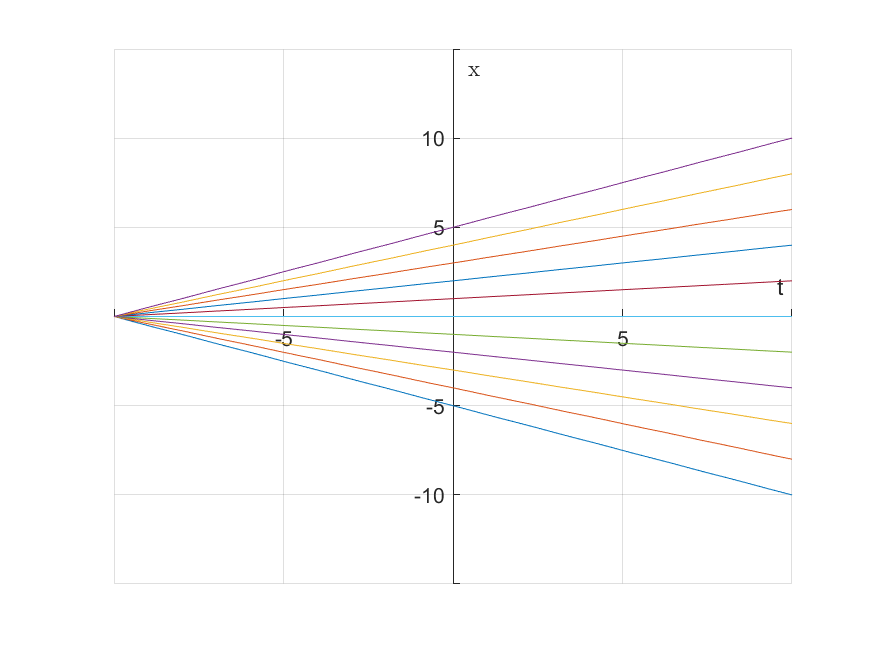
\includegraphics[width=\linewidth]{./SmallOscillations/S8/F3.png}
		\end{subfigure}
		\begin{subfigure}[b]{0.48\linewidth}
			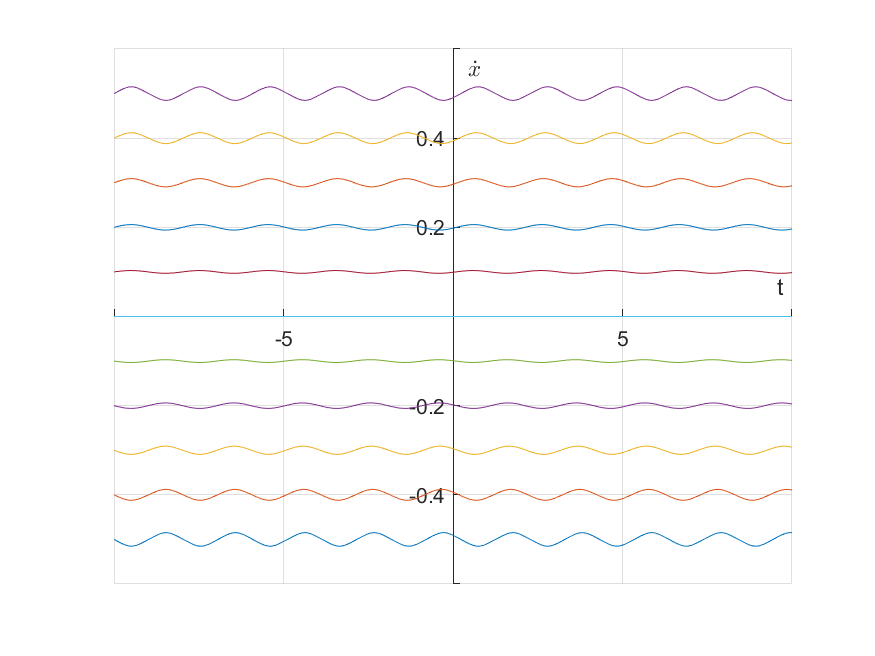
\includegraphics[width=\linewidth]{./SmallOscillations/S8/F4.png}
		\end{subfigure}
	\end{figure}
	
	\begin{figure}[h!]
		\centering
		\begin{subfigure}[b]{0.48\linewidth}
			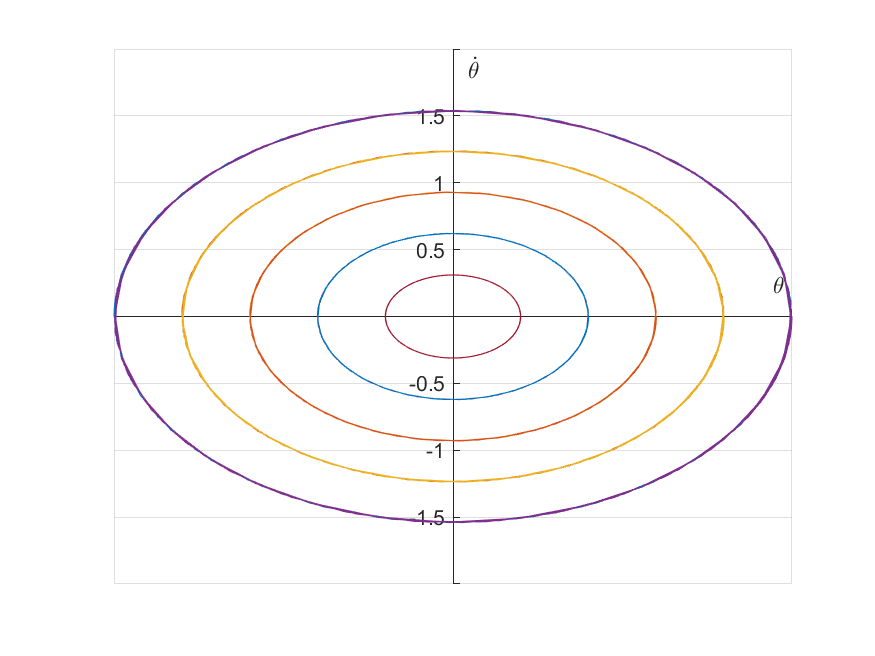
\includegraphics[width=\linewidth]{./SmallOscillations/S8/F5.png}
		\end{subfigure}
		\begin{subfigure}[b]{0.48\linewidth}
			\includegraphics[width=\linewidth]{./SmallOscillations/S8/F6.png}
		\end{subfigure}
	\end{figure}
	\newpage
	
	Case 9:
	Large Bob mass, no initial velocity to support and small initial angular velocity.
	\begin{figure}[h!]
		\centering
		\begin{subfigure}[b]{0.48\linewidth}
			\includegraphics[width=\linewidth]{./SmallOscillations/S9/F1.png}
		\end{subfigure}
		\begin{subfigure}[b]{0.48\linewidth}
			\includegraphics[width=\linewidth]{./SmallOscillations/S9/F2.png}
		\end{subfigure}
	\end{figure}
	
	\begin{figure}[h!]
		\centering
		\begin{subfigure}[b]{0.48\linewidth}
			\includegraphics[width=\linewidth]{./SmallOscillations/S9/F3.png}
		\end{subfigure}
		\begin{subfigure}[b]{0.48\linewidth}
			\includegraphics[width=\linewidth]{./SmallOscillations/S9/F4.png}
		\end{subfigure}
	\end{figure}
	
	\begin{figure}[h!]
		\centering
		\begin{subfigure}[b]{0.48\linewidth}
			\includegraphics[width=\linewidth]{./SmallOscillations/S9/F5.png}
		\end{subfigure}
		\begin{subfigure}[b]{0.48\linewidth}
			\includegraphics[width=\linewidth]{./SmallOscillations/S9/F6.png}
		\end{subfigure}
	\end{figure}
	\newpage
	
	Case 10:
	Large Bob mass, no initial velocity to support and small angular displacement.	
	\begin{figure}[h!]
		\centering
		\begin{subfigure}[b]{0.48\linewidth}
			\includegraphics[width=\linewidth]{./SmallOscillations/S10/F1.png}
		\end{subfigure}
		\begin{subfigure}[b]{0.48\linewidth}
			\includegraphics[width=\linewidth]{./SmallOscillations/S10/F2.png}
		\end{subfigure}
	\end{figure}
	
	\begin{figure}[h!]
		\centering
		\begin{subfigure}[b]{0.48\linewidth}
			\includegraphics[width=\linewidth]{./SmallOscillations/S10/F3.png}
		\end{subfigure}
		\begin{subfigure}[b]{0.48\linewidth}
			\includegraphics[width=\linewidth]{./SmallOscillations/S10/F4.png}
		\end{subfigure}
	\end{figure}
	
	\begin{figure}[h!]
		\centering
		\begin{subfigure}[b]{0.48\linewidth}
			\includegraphics[width=\linewidth]{./SmallOscillations/S10/F5.png}
		\end{subfigure}
		\begin{subfigure}[b]{0.48\linewidth}
			\includegraphics[width=\linewidth]{./SmallOscillations/S10/F6.png}
		\end{subfigure}
	\end{figure}
	\newpage
	
	Case 11:
	Large Bob mass, initial velocity to support and small initial angular velocity.
	\begin{figure}[h!]
		\centering
		\begin{subfigure}[b]{0.48\linewidth}
			\includegraphics[width=\linewidth]{./SmallOscillations/S11/F1.png}
		\end{subfigure}
		\begin{subfigure}[b]{0.48\linewidth}
			\includegraphics[width=\linewidth]{./SmallOscillations/S11/F2.png}
		\end{subfigure}
	\end{figure}
	
	\begin{figure}[h!]
		\centering
		\begin{subfigure}[b]{0.48\linewidth}
			\includegraphics[width=\linewidth]{./SmallOscillations/S11/F3.png}
		\end{subfigure}
		\begin{subfigure}[b]{0.48\linewidth}
			\includegraphics[width=\linewidth]{./SmallOscillations/S11/F4.png}
		\end{subfigure}
	\end{figure}
	
	\begin{figure}[h!]
		\centering
		\begin{subfigure}[b]{0.48\linewidth}
			\includegraphics[width=\linewidth]{./SmallOscillations/S11/F5.png}
		\end{subfigure}
		\begin{subfigure}[b]{0.48\linewidth}
			\includegraphics[width=\linewidth]{./SmallOscillations/S11/F6.png}
		\end{subfigure}
	\end{figure}
	\newpage
	
	Case 12:
	Large Bob mass, initial velocity to support and small angular displacement.	
	\begin{figure}[h!]
		\centering
		\begin{subfigure}[b]{0.48\linewidth}
			\includegraphics[width=\linewidth]{./SmallOscillations/S12/F1.png}
		\end{subfigure}
		\begin{subfigure}[b]{0.48\linewidth}
			\includegraphics[width=\linewidth]{./SmallOscillations/S12/F2.png}
		\end{subfigure}
	\end{figure}
	
	\begin{figure}[h!]
		\centering
		\begin{subfigure}[b]{0.48\linewidth}
			\includegraphics[width=\linewidth]{./SmallOscillations/S12/F3.png}
		\end{subfigure}
		\begin{subfigure}[b]{0.48\linewidth}
			\includegraphics[width=\linewidth]{./SmallOscillations/S12/F4.png}
		\end{subfigure}
	\end{figure}
	
	\begin{figure}[h!]
		\centering
		\begin{subfigure}[b]{0.48\linewidth}
			\includegraphics[width=\linewidth]{./SmallOscillations/S12/F5.png}
		\end{subfigure}
		\begin{subfigure}[b]{0.48\linewidth}
			\includegraphics[width=\linewidth]{./SmallOscillations/S12/F6.png}
		\end{subfigure}
	\end{figure}
	\newpage
	
	Case 12:
	At Large Energies.	
	\begin{figure}[h!]
		\centering
		\begin{subfigure}[b]{0.48\linewidth}
			\includegraphics[width=\linewidth]{./SmallOscillations/Chaotic/F1.png}
		\end{subfigure}
		\begin{subfigure}[b]{0.48\linewidth}
			\includegraphics[width=\linewidth]{./SmallOscillations/Chaotic/F2.png}
		\end{subfigure}
	\end{figure}
	
	\begin{figure}[h!]
		\centering
		\begin{subfigure}[b]{0.48\linewidth}
			\includegraphics[width=\linewidth]{./SmallOscillations/Chaotic/F3.png}
		\end{subfigure}
		\begin{subfigure}[b]{0.48\linewidth}
			\includegraphics[width=\linewidth]{./SmallOscillations/Chaotic/F4.png}
		\end{subfigure}
	\end{figure}
	
	\begin{figure}[h!]
		\centering
		\begin{subfigure}[b]{0.48\linewidth}
			\includegraphics[width=\linewidth]{./SmallOscillations/Chaotic/F5.png}
		\end{subfigure}
		\begin{subfigure}[b]{0.48\linewidth}
			\includegraphics[width=\linewidth]{./SmallOscillations/Chaotic/F6.png}
		\end{subfigure}
	\end{figure}
	\newpage
	
	\section*{References and Acknowledgements}
		\begin{enumerate}
			\item Goldestien, Classical Mechanics
			\item Laundau Lifshiftz, Mechanics
			\item J R Taylor Classical Mechanics
		\end{enumerate}

	We would like to acknowledge our professors, Prof. Krishna Kumar and Prof. Kannabiran Seshasayanan who were a continuous guidance during this process and their exceptional guidance for the same.
	\section*{Authors}
 		Members of Group E
		\begin{itemize}
		\item Pawan 
		\item Rohit Mistry
		\item Ayush Khandelwal
		\end{itemize}

\end{document}
